\chapter{Introduction}
As networks grow larger and more complex, redundancy becomes desirable and necessary.
Adding redundant links always introduces loops to the network.
Switches and hubs respond to broadcast messages by sending them over every port (except for the one the packet was received on).
In conjunction with loops, this behaviour leads to broadcast messages being repeated indefinitely.
With the right network setup, these messages can also multiply exponentially. 
These conditions are called broadcast storms\cite{bstorm}.
Figure~\ref{fig:bc_storm} shows an example of a broadcast storm.
Because of this the Spannning Tree Protocol (STP)\cite{perlman85} was created.
It creates an overlay network, in the shape of a tree, to remove loops from the network.
In this overlay, broadcast storms are not possible anymore.
An example for broadcast propagation in an STP overlay network in Figure~\ref{fig:stp_example}.

\begin{figure}[p]
    \begin{center}
        \begin{subfigure}[b]{0.4\textwidth}
            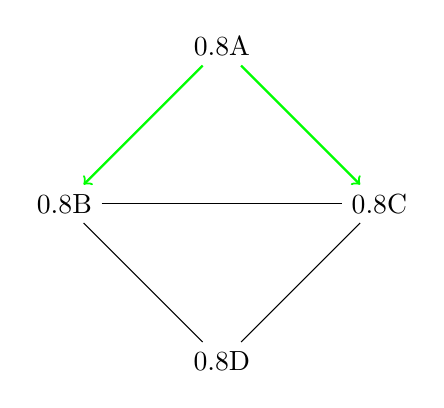
\begin{tikzpicture}
                \node (root) at (4,8) {\switch{0.8}{A}};
                \node (B) at (2,6) {\switch{0.8}{B}};
                \node (C) at (6,6) {\switch{0.8}{C}};
                \node (D) at (4,4) {\switch{0.8}{D}};

                \draw
                (B) edge (C)
                (B) edge (D)
                (C) edge (D);

                \draw[green, thick, ->] 
                (root) edge (B)
                (root) edge (C);
            \end{tikzpicture}
            \caption{Broadcast is sent}
        \end{subfigure}
        \hspace{1cm}
        \begin{subfigure}[b]{0.4\textwidth}
            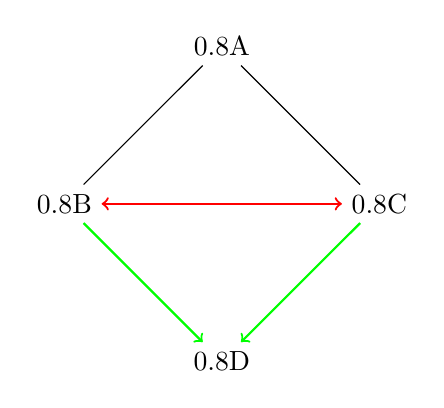
\begin{tikzpicture}
                \node (root) at (4,8) {\switch{0.8}{A}};
                \node (B) at (2,6) {\switch{0.8}{B}};
                \node (C) at (6,6) {\switch{0.8}{C}};
                \node (D) at (4,4) {\switch{0.8}{D}};

                \draw 
                (root) edge (B)
                (root) edge (C);

                \draw[green, thick, ->] 
                (B) edge (D)
                (C) edge (D);

                \draw[red, thick, <->]
                (B) edge (C);
            \end{tikzpicture}
            \caption{Broadcast is propagated}
        \end{subfigure}
    \end{center}
    
    \begin{center}
        \begin{subfigure}[b]{0.4\textwidth}
            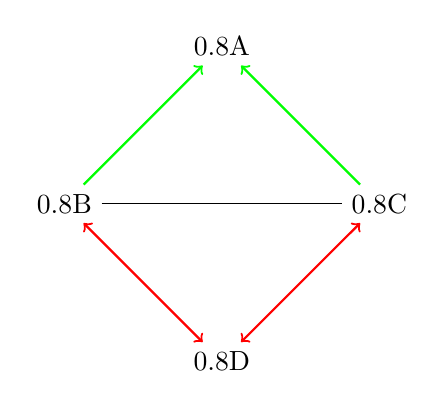
\begin{tikzpicture}
                \node (root) at (4,8) {\switch{0.8}{A}};
                \node (B) at (2,6) {\switch{0.8}{B}};
                \node (C) at (6,6) {\switch{0.8}{C}};
                \node (D) at (4,4) {\switch{0.8}{D}};

                \draw
                (B) edge (C);

                \draw[green, thick, ->]
                (B) edge (root)
                (C) edge (root);

                \draw[red, thick, <->]
                (B) edge (D)
                (C) edge (D);

            \end{tikzpicture}
        \caption{Broadcasts start multiplying}
        \end{subfigure}
        \hspace{1cm}
        \begin{subfigure}[b]{0.4\textwidth}
            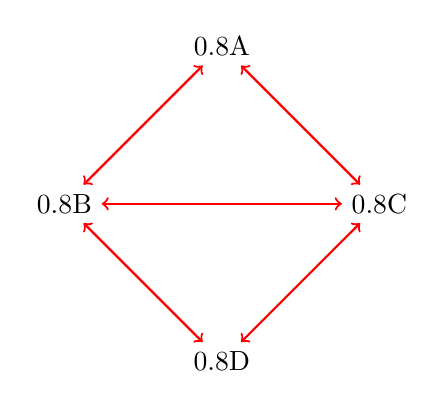
\begin{tikzpicture}
                \node (root) at (4,8) {\switch{0.8}{A}};
                \node (B) at (2,6) {\switch{0.8}{B}};
                \node (C) at (6,6) {\switch{0.8}{C}};
                \node (D) at (4,4) {\switch{0.8}{D}};

                \draw[red, thick, <->]
                (root) edge (B)
                (root) edge (C)
                (B) edge (C)
                (B) edge (D)
                (C) edge (D);
            \end{tikzpicture}
        \caption{Broadcast storm}
        \end{subfigure}
    \end{center}
    \caption{An example of a broadcast storm}
    \label{fig:bc_storm}
\end{figure}

\begin{figure}[p]
    \begin{centering}
        \begin{subfigure}[b]{0.4\textwidth}
            \begin{tikzpicture}
                \node (root) at (4,8) {\switch{0.8}{A}};
                \node (B) at (2,6) {\switch{0.8}{B}};
                \node (C) at (6,6) {\switch{0.8}{C}};
                \node (D) at (4,4) {\switch{0.8}{D}};

                \draw[green, thick, ->]
                (root) edge (B)
                (root) edge (C);

                \draw
                (B) edge (D);
            \end{tikzpicture}
            \caption{Broadcast is sent}
        \end{subfigure}
        \hspace{1cm}
        \begin{subfigure}[b]{0.4\textwidth}
            \begin{tikzpicture}
                \node (root) at (4,8) {\switch{0.8}{A}};
                \node (B) at (2,6) {\switch{0.8}{B}};
                \node (C) at (6,6) {\switch{0.8}{C}};
                \node (D) at (4,4) {\switch{0.8}{D}};

                \draw[green, thick, ->]
                (B) edge (D);

                \draw
                (root) edge (B)
                (root) edge (C);
            \end{tikzpicture}
            \caption{Broadcast propagation done}
        \end{subfigure}    
    \end{centering}
    \caption{Broadcast propagation in an STP network}
    \label{fig:stp_example}
\end{figure}
For this thesis, we will only talk about switches.
Hubs, while still existent, are hardly ever used and not STP capable.
We will also refer to switches as bridges, in order to be compliant with STP nomenclature.\\

Networks where STP is utilized are usually quite large.
Additionally, changes and outages are hidden by STP and redundant links in the network.
This can make it hard to keep track of the current network layout.
Debugging STP configurations is also a difficult and time consuming task.
It is possible to check STP configurations via the Simple Network Management Protocol (SNMP).
However, this requires an administrator to connect to every single bridge and collect the STP information manually.
While there are tools to automate this, they rely primarily on SNMP, which may not be supported by all bridges in the network.\\

The aim of this project was to create a versatile tool for STP visualization.
This tool had the following requirements:
\begin{itemize}
    \item \textbf{STP only}: the tool could only rely on STP packets
    \item \textbf{Low traffic}: the tool should create as low a traffic as possible
    \item \textbf{Passive}: the tool could not provoke any changes in the network and only use packets obtained passively
    \item \textbf{Distributed}: the tool is to be run on multiple nodes, to send information to a central server where everything is pieced together
    \item \textbf{Low hardware load}: the tool must run on simplistic hardware (e.g. a Raspberry Pi) or on a regular PC without slowing it down noticeably
    \item \textbf{No maintenance}: once set up, the tool must not require any maintenance (except when updating to a new version)
    \label{requirements}
\end{itemize}

%TODO: do overview
